%!TEX root = ../thesis.tex

% TABLE: SM Summary
%   https://en.wikipedia.org/wiki/File:Electroweak.svg
%   https://commons.wikimedia.org/wiki/File:Standard_Model.svg
%   https://en.wikipedia.org/wiki/Mathematical_formulation_of_the_Standard_Model#Field_content_in_detail
\begin{table}[p]
\vspace*{-6mm}
\centering
\caption{
Summary of the representation and quantum numbers SM fields.
Bold numbers indicate the dimension of the representation under the respective gauge group.
}\label{tab:SM_symmetries}
\def\arraystretch{1.3}
\def\vsdb{\rule[-15pt]{0pt}{36pt}} % vertical space for doublet
\begin{tabular}{llc@{\extracolsep{\tabcolsep}}c@{\extracolsep{4pt}}c@{\extracolsep{\tabcolsep}}c@{\extracolsep{1.5\tabcolsep}}c}
  \hline
  %Field name  & Symbol      & $\SU[C]{3}$ & $\SU[L]{2}$ & $T_3$ & $\YW/2$ & $Q = T_3 + \YW/2$ \\
  \multirow{2}{*}{Field name}
        & \multirow{2}{*}{Symbol}
               & \multicolumn{2}{c}{Representations} & \multicolumn{3}{c}{Quantum numbers} \\
                 \cline{3-4}                           \cline{5-7}
        &      & $\SU[C]{3}$ & $\SU[L]{2}$ & $T_3$ & $\YW/2$ & $Q = T_3 + \YW/2$ \\
  \hline
  \vsdb % add vertical space above & below
  Quark doublet
        & $\ff{Q}{L} = \db{\ff{u}{L}}{[1pt]\ff{d}{L}}$
               & \textbf{3}  & \textbf{2} & $\db{+\frac{1}{2}}{[2pt]-\frac{1}{2}}$
                                                   & $+\frac{1}{6}$
                                                             & $\db{+\frac{2}{3}}{[2pt]-\frac{1}{3}}$ \\[2mm]
  Up-quark singlet
        & $\ff{u}{R}$  & \textbf{3}  & \textbf{1} & $+\frac{2}{3}$
                                                   & $+\frac{2}{3}$
                                                             & $+\frac{2}{3}$ \\
  Down-quark singlet
        & $\ff{d}{R}$  & \textbf{3}  & \textbf{1} & $-\frac{1}{3}$
                                                   & $-\frac{1}{3}$
                                                             & $-\frac{2}{3}$ \\
  \vsdb % add vertical space above & below
  Lepton doublet
        & $\ff{L}{L} = \db{\ff{\nu}{L}}{[1pt]\ff{e}{L}}$ 
                       & \textbf{1}  & \textbf{2} & $\db{+\frac{1}{2}}{[2pt]-\frac{1}{2}}$
                                                   & $-\frac{1}{2}$
                                                             & $\db{\phmin0}{-1}$ \\[2mm]
  Lepton singlet
        & $\ff{e}{R}$  & \textbf{1}  & \textbf{1} & $\phmin0$
                                                   & $-1$    & $-1$ \\
  \hline
  Gluon field
        & $G^a_\mu$    & \textbf{8}  & \textbf{1} & $\phmin0$
                                                   & $\phmin0$ & $\phmin0$ \\
  \rule[-19pt]{0pt}{42pt}% % add vertical space above & below
  Weak gauge field
        & $W^i_\mu = \db{W^+_\mu}{W^-_\mu\\W^3_\mu}$
                       & \textbf{1}  & \textbf{3} & $\db{+1}{-1\\\phmin0}$
                                                   & $\phmin0$ & $\db{+1}{-1\\\phmin0}$\\
  Hypercharge field
        & $B_\mu$
                       & \textbf{1}  & \textbf{1} & $\phmin0$
                                                   & $\phmin0$ & $\phmin0$ \\
%  Weak gauge bosons
%        & $\db{W^+_\mu}{W^-_\mu\\Z^0_\mu}$
%               & \textbf{1}  & \textbf{3} & $\db{+1}{-1\\0}$
%                                                   & \phmin0 & $\db{+1}{-1\\\phmin0}$\\
%  Photon
%        & $A^a_\mu$    & \textbf{1}  & \textbf{1} & $\phmin0$
%                                                   & $\phmin0$ & $\phmin0$ \\
  \hline
  \vsdb % add vertical space above & below
  Higgs doublet
        & $\Phi = \db{\phi^+}{[1pt]\phi^0}$
               & \textbf{1}  & \textbf{2} & $\db{+\frac{1}{2}}{[2pt]-\frac{1}{2}}$
                                                   & $+\frac{1}{2}$
                                                             & $\db{+1}{\phmin0}$ \\[2mm]
  \vsdb % add vertical space above & below
  Conjugate Higgs doublet
        & $\Phi^\mathrm{c} = \db{\phi^{0*}}{[1pt]\phi^-}$
               & \textbf{1}  & \textbf{2} & $\db{+\frac{1}{2}}{[2pt]-\frac{1}{2}}$
                                                   & $-\frac{1}{2}$
                                                             & $\db{\phmin0}{-1}$ \\[2mm]
  \hline
\end{tabular}
\end{table}


% FIG: SM Summary
\begin{figure*}[p]
  \vspace*{-10mm}
  \centerline{
    \includegraphics[height=0.56\linewidth,page=5]{fig/intro/SM_isospin_weak.pdf}
    \includegraphics[height=0.56\linewidth,page=4]{fig/intro/SM_isospin_weak.pdf}
  }
  \caption{
Graph of the $(T_3,\YW/2)$ quantum numbers.
  }\label{fig:SM_quantum_numbers_fermions}
  \vspace*{-6mm}
\end{figure*}
